\documentclass[12pt,a4paper,titlepage]{article}

\usepackage{amsmath}
\usepackage{latexsym}
\usepackage{amssymb}
\usepackage{amstext}
\usepackage{fancyhdr}

\usepackage{graphicx,picinpar,emlines2,epsf}

\usepackage{color}
\usepackage{titlesec}

\usepackage{./texcode/MCM}
\usepackage{lastpage}
\setcounter{page}{178}

\setlength{\textwidth}{13.1cm}
\begin{document}

\setlength{\parindent}{0pt} \setlength{\parskip}{2ex plus 0.5ex
minus 0.2ex}
\title{A Convenient Truth: A model for sea level rise forecast}
\author{Team \# 3694}
\date{February 18, 2008}

\maketitle


\fancyhead{} \pagestyle{fancy} \lhead{Team \# 3694} \rhead{Page
\thepage\ of \pageref{LastPage}} \setlength{\headrulewidth}



\section{Introduction}
Strong evidence of a global warming trend exists, and powerful
models have been created to estimate future climate. Temperatures
have increased by about $0.5\,^{\circ}\mathrm{C}$ over the last 15
years, and global temperature is at its highest level in the past
millennium . Although the warming trend is quite evident, the
consequences of such wide scale climate change are still poorly
understood. One of the most-feared consequences of global warming
is sea level rise, and for good reason. TOPEX/Poseidon satellite
altimeter indicates that sea levels rose $3.2\pm0.2 mm$ annually
during 1993-1998 . Indeed, Titus et al estimate that a 1 meter
rise in sea levels could cause \$270-475 billion in damages in the
United States alone.

A number of complex factors underlie sea level rise. Thermal
expansion of water due to temperature changes has long been
implicated as the major component of sea level rise; however,
recent studies have shown that thermal expansion alone cannot
account for a majority of the observed increases . Mass balance of
large ice sheets, in particular the Greenland Ice Sheet, is now
believed to play a major role in sea level. The mass balance is
controlled by two major processes, accumulation (influx of ice to
the sheet) and ablation (loss of ice from the sheet) .
Accumulation is primarily the result of snowfall; ablation is a
result of sublimation and melting.

Contrary to popular belief, however, floating ice does not play a
significant role in sea level rise. By Archimedes' Principle, the
volume increase $\Delta V$ of a body of water with density
$\rho_{ocean}$ due to melting of floating ice of weight $W$
(assumed to be freshwater, with liquid density $\rho_{water}$) is
given by

\[
\Delta V=W(\frac{1}{\rho_{water}}-\frac{1}{\rho_{ocean}})
\]

The density of seawater is approximately 1024.8 $kg/m3$ ; the mass
of the Arctic sea ice is approximately $2 \times 10^{13} kg$ .
Thus, the volume change if all of the Arctic sea ice melted is
given by:

\[
\Delta
V=2\times10^{13}kg(\frac{1}{1000kg/m^3}-\frac{1}{1024.8kg/m^3})=4.84\times10^8m^3
\]

Approximating that 360 $Gt$ of water causes a rise of 1 $mm$ in
sea level ,

\[
4.84\times10^8m^3\cdot\frac{1000kg}{m^3}\cdot\frac{1Gt}{9.072\times10^{11}kg}\times\frac{1mm}{360Gt}=0.0015mm
\]

This small change in sea level is inconsequential for our model,
since the accuracy is well below one thousandth of a millimeter.

We also neglect the contribution of Antarctic Ice Sheet because
its overall effect on sea level rise is minimal and difficult to
quantify. Between 1978 to1987, satellite-borne microwave
radiometer data indicated that Arctic ice decreased by 3.5\%,
while Antarctic ice showed no statistically significant changes .
Cavalieri et al projected minimal melting in the Antarctic over
the next 50 years . For this reason, only the Greenland Ice Sheet
is considered in the model.

Several models already exist for mass balance and for thermal
expansion. However, these models are very complex with respect to
many variables, and often disagree with each other (see for
example and ). We wish to develop a model based on simple physical
processes, as solely a function of temperature and time. In this
way the analysis of the effects of the warming is simplified, and
the dependence of sea level rise on temperature becomes evident.
Furthermore, we develop a model that can be extended to several
different temperature forcings, allowing us to compare firsthand
the effect of carbon emissions on sea level rise.

\subsection{Model Overview}

A deeper understanding of ice sheet melting would provide valuable
insight into sea level rise. By creating a framework that
incorporates the contributions of ice sheet melting and thermal
expansion, we can estimate global mean sea level over a 50-year
time period. The model achieves several important objectives :

\begin{enumerate}

\item Accurately fits past sea level rise data

\item Provide enough generality to predict sea level rise over a
50-year span

\item Compute sea level increases for Florida as a function of
solely global temperature and time

\end{enumerate}

Ultimately, the model predicts consequences to human populations.
In particular, we analyze the impact of sea level rise on the
state of Florida, which many consider particularly vulnerable due
to its generally low elevation and proximity to the Atlantic
Ocean. From this analysis, we assess possible strategies to
minimize damage as a result of sea level rise due to global
warming.

\subsection{Assumptions}

In order to streamline our model we have made several key
assumptions.

\begin{enumerate}

\item \textit{The sea level rise is primarily due to two factors}, the
balance of accumulation/ablation of the Greenland Ice Sheet and
the thermal expansion of the ocean. This ignores the contribution
of processes such as calving and direct human intervention, which
are difficult to model accurately and have minimal effect on sea
level rise .

\item \textit{The air is the only heat source for melting the ice}.
Greenland's land is permafrost, and because of large amounts of
ice on its surface it is assumed at a relatively constant
temperature. This allows us to use convection as a mode of heat
transfer.

\item \textit{The temperature within the ice changes linearly at the
steady-state}. This assumption allows us to solve the heat
equation for Neumann conditions. By subtracting the steady-state
term from the heat equation, we can solve for the homogeneous
boundary conditions.

\item \textit{Sublimation and melting processes do not interfere with each
other}. This assumption drastically simplifies the computation
needed for the model since sublimation and melting can be
considered separately. Additionally, the assumption is very
reasonable. Sublimation primarily occurs at below freezing
temperatures, a condition during which melting does not normally
occur. Thus, the two processes are temporally isolated as in our
model.

\item \textit{The surface of the ice sheet is homogeneous with regards to
temperature, pressure, and chemical composition}. This assumption
is necessary because high-resolution spatial temperature data for
Greenland cannot be obtained in our framework. Additionally, we
lack the computational resources and time to simulate such a
variation, which would require the use of finite element methods
and mesh generation for a complex topology.

\end{enumerate}

\subsection{Defining the problem}

Let $M$ denote the mass balance of the Greenland Ice Sheet. Given
a temperature forcing function, we must quantitatively estimate
the sea level increases $SLR$ that occur as a result. These
increases are a sum of $M$ and thermal expansion $TE$ effects,
corrected for local trends. Further, we must quantitatively and
qualitatively the long-term (50 years) effect on Florida's major
cities and metropolitan areas from global warming, as a result of
high $SLR$. This analysis can be used to make recommendations as
to how to best prepare for and reduce $SLR$ effects.

\section{Methods}

\subsection{Mathematically Modeling Sea Level Rise}

Sea level rise results mostly from mass balance of the Greenland
Ice Sheet and thermal expansion due to warming. In order to model
sea level increases, a mass balance model and thermal expansion
model are used, as well as other post-computation effects. The
logic of the simulation process is detailed in Figure 1.

\begin{figure}[!htb]
\centering
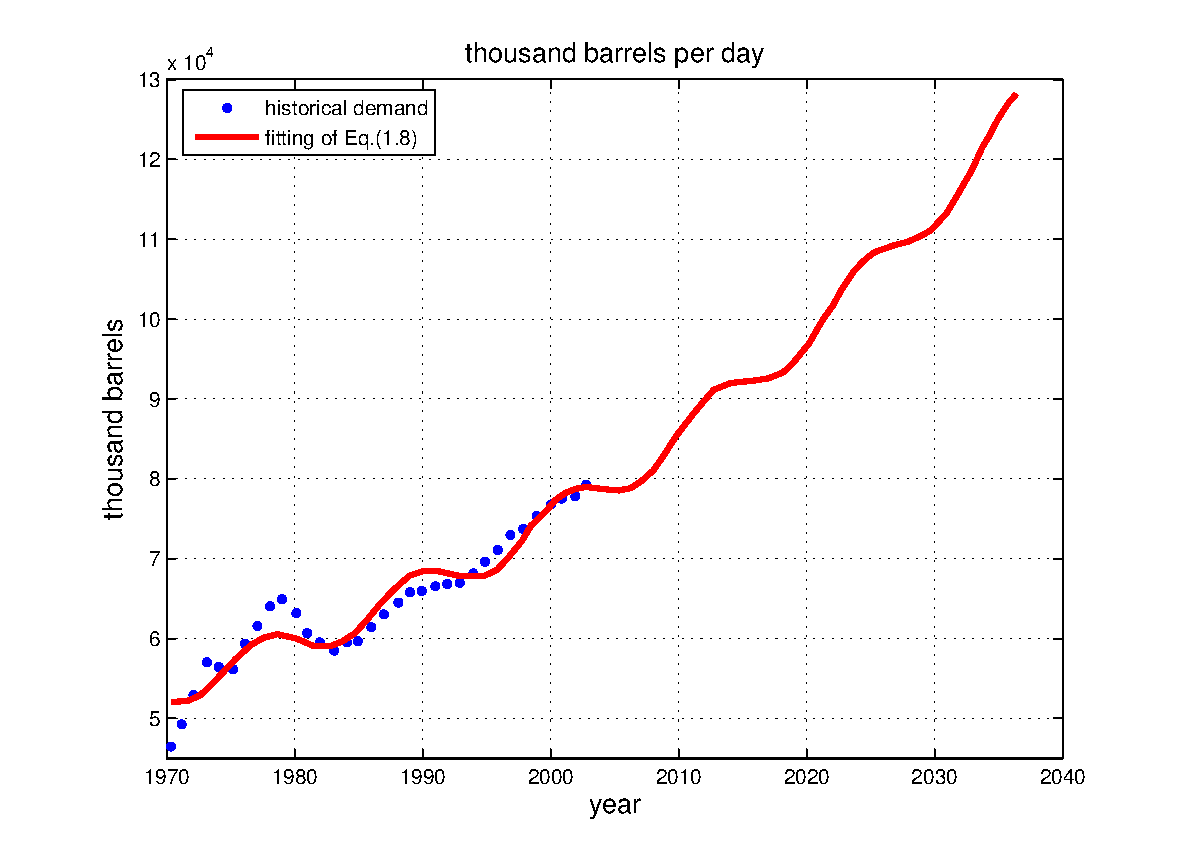
\includegraphics[width=0.55\textwidth]{fig01.eps}
\caption{Simulation flow diagram}
\end{figure}

\subsection{Temperature Data}

Temperature data is the sole forcing in our model and thus shall
be considered carefully. Because we needed to model several
different scenarios, our temperature data must include several
scenarios that are very controlled and only differ in one
variable. Further, the temperature data must be of very good
quality and provide the correct temporal resolution for our
simulation. For these reasons, we decided to use a Global Climate
Model (GCM) to create our own temperature data, using input
forcings that we could easily control. Because of limited
computational power and time restrictions, we chose the EdGCM .
EdGCM is a fast model for educational purposes. The program is
based on the NASA GISS model for climate change. The program fit
all of our needs; in particular, the rapid simulation (about 10
hours for a 50 year climate simulation) allowed us to analyze
several different temperature scenarios.

The temperature scenarios we analyzed incorporate the three
estimates of carbon emissions resulting from the IPCC Third
Assessment Report (TAR)-the low, high, and medium projections in
the IS92 series. The IS92e(high), IS92a (intermediate), and the
IS92c(low) scenarios were all closely approximated using the tools
in EdGCM. These approximated carbon forcings are shown in
graphical form in Figure 2. All other forcings were kept at
default according to the NASA GISS model. Three time series for
global surface air temperature were obtained in this fashion.

\begin{figure}[!htb]
\centering
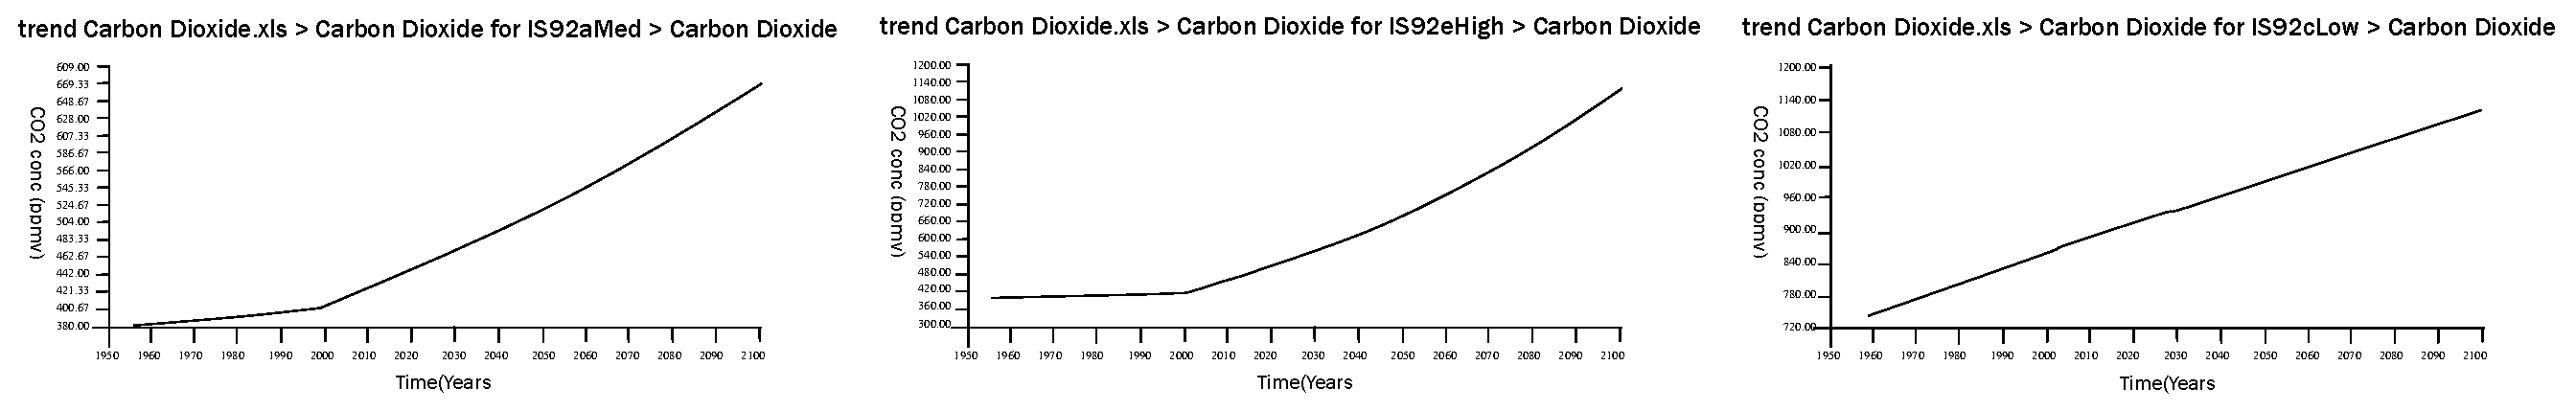
\includegraphics[width=1\textwidth]{fig02.eps}
\caption{Carbon Dioxide Forcings for the EdGCM Models}
\end{figure}

One downside to the EdGCM is that it can only output global
temperature changes . Regional temperature changes are calculated,
but are difficult to access and have low spatial accuracy.
However, according to Chylek et al , the relationship between
Greenland temperatures and global temperatures is
well-approximated by

\[
\Delta T_{Greenland}=2.2\times\Delta T_{global}
\]

This result is shown by Chylek et al for regions unaffected by the
NAO and is predicted by climate model outputs.

\subsection{The Ice Sheet}

The ice sheet is modeled as a simplified rectangular box. Each
point on the upper surface of the ice sheet is assumed at constant
temperature, $T_a$. This is because our climate model does not
have accurate spatial resolution for areas in Greenland, so the
small temperature differences are ignored. The lower surface, the
permafrost layer, has constant temperature $T_l$. A depiction of
the ice sheet model is shown in Figure 3.

\begin{figure}[!htb]
\centering
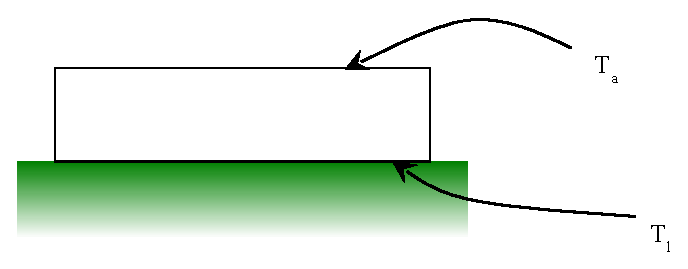
\includegraphics[width=0.6\textwidth]{fig03.eps}
\caption{Carbon Dioxide Forcings for the EdGCM Models}
\end{figure}

To compute heat flux and thus melting and sublimation through the
as an infinite number of differential volumes, shown in Figure 4.

\begin{figure}[!htb]
\centering
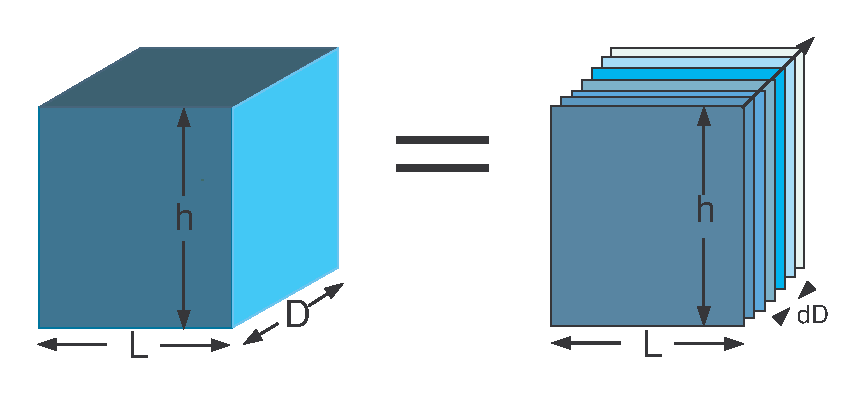
\includegraphics[width=0.6\textwidth]{fig04.eps}
\caption{Differential volumes of the ice sheet}
\end{figure}

Initially, the height h is calculated using data provided by
Williams et al .

\[
h=\frac{Vol_{ice}}{Surface_{ice}}=\frac{2.6\times10^{6}km^3}{1.736\times
10^3km^2 }=1498km
\]

The primary mode of sea level rise in our model is through mass
balance. Mass balance is calculated by subtracting the amount of
ablation by the amount of accumulation. Accumulation, the addition
of ice to the ice sheet, is primarily in the form of snowfall.
Ablation is primarily the result of two processes, sublimation and
melting.

\subsection{Mass Balance-Accumulation}

First we model accumulation. Huybrechts et al showed that the
temperature of Greenland is not high enough to melt significant
amounts of snow. Furthermore, Knight showed empirically that rate
of accumulation is well-approximated by a linear relationship with
time, and that accumulation over Greenland continental ice is 0.30
m/year. Thus, the accumulation rate is 0.025 m/month. In terms of
mass balance,

\[
M_{ac}=0.025LD
\]

where the product $LD$ the surface area of the ice sheet.


\subsection{Mass Balance - Ablation }

We then model the two parts of ablation, sublimation and melting.

Sublimation rate (mass flux) is given by:

\[
S_0=e_{sat}(T)(\frac{M_w}{2\pi RT})^{1/2}
\]


where $M_w$ is the molecular weight of water. This expression can
be derived from the ideal gas law and the Maxwell-Boltzmann
distribution . Substituting Buck's expression for $e_{sat}$, we
obtain:

\[
S_{0}=6.1121\times
e^{[\frac{(18.678-T/234.5)T}{257.14+T}]}[\frac{M_w}{2\pi
R(T+273.15)}]^{\frac{1}{2}}
\]

Buck's equation is applicable over a large range of temperatures
and pressures, including the environment of Greenland. The
approximation fails at extreme temperatures and pressures but is
computationally simple (relatively). To convert mass flux into
rate of thickness change of the ice, we divide the mass flux
expression by the density of ice. Thus we can express rate of
height change as follows:

\[
S_h=\frac{6.1121\cdot d}{\rho_{ice}}\cdot
e^{[\frac{(18.678-T/234.5)T}{257.14+T}]}[\frac{M_w}{2\pi
R(T+273.15)}]^\frac{1}{2}
\]

where $d$ is the deposition factor, given by $d
=(1-\textrm{deposition rate})=0.01$. This term is needed because
sublimation and deposition are in constant equilibrium. With the
sublimation rate expression, it is now trivial to find the
thickness of the ice sheet after one timestep of the computational
model. Indeed, the new thickness due to ablation via sublimation
is given by:

\[
S(t)=h-S_h\cdot t
\]

where $h$ is the current thickness of the ice sheet and $t$ is the
elapsed time after one timestep. Substituting for $S_h$ with the
expression we derived and substituting for the known value of the
molecular weight of water yields

\[
S(t)=h-\frac{6.1121\times10^{-2}t}{\rho_{ice}}\cdot
e^{[\frac{(18.678-T/234.5)T}{257.14+T}]}[\frac{0.0003448}{(T+273.15)}]^\frac{1}{2}
\]

This equation governs the sublimation of the ice.

To model melting, the second component of ablation, we apply the
heat equation. The heat equation governs the relationship

\[
U_t(x,t)=kU_{xx}(x,t)
\]

where $k=0.0104$ is the thermal diffusivity of the ice . In order
to solve the heat equation for the Neumann conditions, we assume a
steady-state $U_s$ with the same boundary conditions as $U$ and
that is independent of time. The residual temperature $V$ has
homogeneous boundary conditions and initial conditions found by
$U$-$U_s$. Thus we can rewrite the heat equation as:

\[
U(x,t)=V(x,t)+U_s(x,t)
\]

The steady-state solution of the heat equation is given by:

\[
U_s=T_l+\frac{T_a-T_l}{S(t)}x
\]

subject to the constraints $0<x< S(t)$ and $0<t<1$ month. The
following equations follow directly from the heat equation as
well:

$V_t(x,t)=kV_{xx}+f$,where $f$ is a forcing term.

$V(0,t)=V(S(t),t)=0$(necessary conditions for the homogeneous
boundary equations)

Since no external heat source is present and temperature
distribution only depends on heat convection, we take the forcing
term $f = 0$. To calculate change in mass balance on a monthly
basis, we solve analytically using separation of variables:

\[
V(x,t)=\frac{a_0}{2}+\sum^\infty}_{n=1}{a_ne^{-n^2\pi^2t/s^2}\cos(\frac{n\pi
x}{s})}
\]

where

\[
a_0=\frac{2}{s}\int^s_0(T_l+\frac{T_a-T_l}{s}x)dx=2T_l+T_a-T_l=T_l+Ta
\]

 and

\[
a_0=\frac{2}{s}\int^s_0(T_l+\frac{T_a-T_l}{s}x)\cos(\frac{n\pi
x}{s})dx
\]

\[
=(\frac{s}{n\pi})^2(\cos(n\pi)-1)=(\frac{s}{n\pi})^2((-1)^n-1)
\]

Therefore,

\[
V(x,t)=\frac{T_l+T_a}{2}+\sum^\infty_{n=1}\frac{2(T_a-T_c)}{(n\pi)^2}((-1)^n-1)e^{-n^2\pi^2t/s^2
}\cos(\frac{n\pi x}{s})
\]

Having found $V(x,t)$ and $U_s(x,t)$, we obtain an expression for
$U(x,t)$:
\[
U(x,t)=V(x,t)+U_s(x,t)
\]

Since $U$ is an increasing function of $x$, and for $x>k$, $U(x,t)
>0$ for fixed $t$, the ice will melt for $k<x<h$. Thus, we seek
the solution to $U(k,t)=0$ for $k$ to determine ablation.
Computationally, we solve this expression using the first 100
terms of the Fourier series expansion and the MATLAB function
$fzero$. The solution of this equation for k is the primary
computational step for the MATLAB simulation (see Appendix A). The
new value of $k$ is used to renew $h$ as the new thickness of the
ice sheet, and a consequent time step can begin calculation.

With these two components we can now finalize an expression for
ablation and apply it to a computational model. The sum of the
infinitesimal changes in ice sheet thickness for each differential
volume gives the total change in thickness. To find these changes,
we first note that

\[
\textrm{\textit{Mass Balance Loss Due to Sublimation}} =(h-S)LD
\]

\[
\textrm{\textit{Mass Balance Loss Due to Melting}}=(S-k)LD
\]

where the product $LD$ is the surface area of the ice sheet. Note
that in these equations, the "mass balance" refers to net volume
change. Thus, ablation is given by

\[
M_{ab}= (h+S)LD+(S-k)LD=(h-k)LD
\]

\subsection{Mass Balance and Sea Level Rise}

Combining accumulation and ablation into an expression for mass
balance, we have

\[
M=M_{ac}-M_{ab}=0.025LD-(h-k)LD
\]

Relating this to sea level rise, we use the approximation 360$Gt$
water = 1$mm$ sea level rise. Thus,

\[
SLR_{mb}=M\cdot\rho_{ice}\cdot\frac{1mm}{360Gt}
\]

which quantifies the sea level rise due to mass balance.

\subsection{Thermal Expansion}

A second mode of sea level rise is also considered: thermal
expansion due to warming. According to various literature ,
thermal expansion of the oceans due to increase in global
temperature will contribute a significant portion of the rise in
future sea level, at least as much as melting of polar ice for the
current century , . Therefore, we incorporated this component into
our model for further accuracy and a more comprehensive
understanding.

Thermal expansion operates depending on various factors.
Temperature plays the primary role, but the diffusion of radiated
heat, mixing of the ocean, and various other complexities
concerning ocean dynamics must be accounted for a fully accurate
description of the phenomenon. These factors are often quite
difficult to understand with a high degree of certainty. The model
used here adapts the model of Wigley et al . Based on standard
greenhouse-gas emission projections and a simple
upwelling-diffusion model, the dependency of the model can be
narrowed to a single variable, temperature, using an empirical
estimation:

\[
\Delta z=6.89\Delta Tk^{0.221}
\]

where $\Delta z$ is the change in sea level due to thermal
expansion given in centimeters, $\Delta T$ is the change in global
temperature, and $k$ is the diffusivity.

The reader is encouraged to consult for further investigation of
the upwelling-diffusion model.

\subsection{Localization}

A final correction must be added to the simulation. Although the
literature in general cites an increase in the mean sea level for
the past century and indicates that melting of polar ice and other
various effects associated with global warming will force the
trend, the effect varies regionally rather significantly. The
local factors often cited include land subsidence, compaction, and
delayed response to the warming, to name a few . Fully
understanding the influences of these factors on sea level
increase is often a daunting task. We thus assume that previous
patterns of local sea level variation will continue to influence,
yielding the relationship

\[
\textrm{local(t)}=\textrm{normalized}(t)+\textrm{trend}(t-2008)
\]

where $local(t)$ is the expected sea level rise at year t given in
centimeters, $normalized(t)$ is the estimate of expected rise in
global sea level change relative to the historical rate, at year
$t$, and $trend$ is the current rate of sea level change at the
locale of interest. The normalization prevents from double
counting the contribution from global warming.

In our model, the rates of sea level change are averaged over data
given for Florida in to give the $trend$. This is reasonable
because the differences between the rates in Florida are fairly
small. The $normalized(t)$ at each year is obtained by:

\[
\textrm{global}(t)-\textrm{historical rate}(t-2008)
\]

where $global(t)$ is the expected sea level rise at year t from
our model and historical rate is chosen uniformly over the range
taken from .

For a detailed description of the model, the reader may consult .

\subsection{Simulating Costs of Sea Level Rise to Florida}

Rising sea levels could submerge coastal areas of Florida that are
near current sea level. To model the submersion of regions of
Florida due to sea level rise, a raster matrix of elevation values
for various latitude and longitude was created. The matrix was
created on MATLAB using 30-arc-second global elevation data
(GTOPO30), created in 1996 . The 30-arc-second resolution
corresponds to about 1 $km$; however, in order to yield a more
practical matrix, the resolution was lowered to 1 minute of arc
(approximately 2 $km$). The vertical resolution of the GTOPO30
data is much greater than 1 meter and thus accurate models could
not easily be produced. In order to more accurately model the low
coastal regions, the matrix generation code identified potential
sensitive areas and submitted these locations to the National
Elevation Dataset (NED) for refinement. NED is updated bimonthly,
but its large size and download restrictions restrict its use to
only these sensitive areas. The vertical resolution of NED is very
high, depending on the region surveyed. Although Florida NED data
has a mean error of $\pm4.3$ $ft$, areas of low elevation have
especially high resolution . These adjustments finalized the
elevation data raster matrix for use in the sea level increase
simulation.

The effect of this sea level rise on human populations was
measured by incorporating city geospatial coordinates and
population into the simulation. Geospatial coordinates were
obtained from the GEOnames Query Database maintained by the
National Geospatial Intelligence Agency . Population data was
obtained from the US Census Bureau 2000 Datasets . All major
metropolitan areas and several large cities were analyzed,
encompassing both interior (e.g.,Gainesville) and coastal (e.g.,
Miami). The population of the metropolitan areas was equally split
into the principle cities in order to streamline the simulation
(see Appendix D).

The sea level rise calculated from our model was used as input for
the submersion simulation. The simulation script subtracts the sea
level increase from the existing elevation data. Pixels with
elevations below sea level are checked to determine whether they
are connected (directly or indirectly through other submerged
areas) to the Atlantic Ocean or the Gulf of Mexico. This way,
interior areas not connected to the oceans are not identified as
submerged regions. If rising sea level submerges pixels that form
part of a city or metropolitan area, the population is considered
to be "displaced." A key limitation of the model is that the
population is considered to be concentrated in the principal
cities of the metropolitan areas, so a highly accurate population
count cannot be assessed. This simplification of the model allows
the quick display of which cities are threatened by rising sea
levels without the complexity of a continuous population
distribution. Additionally, high-resolution population
distribution data is difficult to find and thus cannot be easily
utilized.

The model was checked for realism at several different scenarios
of sea level rise. First, the extreme case of 0 meter sea level
rise was examined. In this case, no cities should be submerged and
no population or land area should be affected. These expectations
are confirmed in Figure 5. The case of 10 meter sea level rise was
also analyzed. This is slightly higher than the sea level increase
estimate if all of the Greenland Ice Sheet melted (approximately 7
meters). Many cities should be submerged, especially in the low
elevation regions in southern Florida. This is confirmed by the
output, shown in Figure 5. Finally, 100 meter sea level rise was
analyzed to check robustness of the simulation. Most of Florida
should be submerged, since it is a relatively low elevation state.
This is also confirmed by Figure 5; note the mountainous regions
of North Florida that are still above water.

\begin{figure}[!htb]
\centering
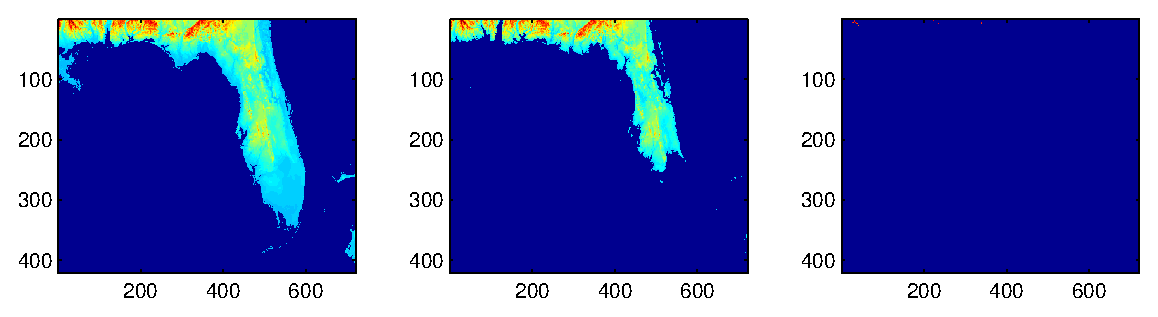
\includegraphics[width=1\textwidth]{fig05.eps} \caption{Graphical effects of 0, 10, and
100 meter sea level rise.}
\end{figure}


\section{Results}

\subsection{Output Sea Level Rise Data}

The program was run with MATLAB script
\textit{massbalance\_sim2.m}, for the IS92e (high), IS92a
(intermediate), and IS92c (low) carbon emissions models. Complete
code is given in Appendix A.

The program produced a smooth trend in sea level increase for each
of the three forcings, shown in Figure 6.

\begin{figure}[!htb]
\centering
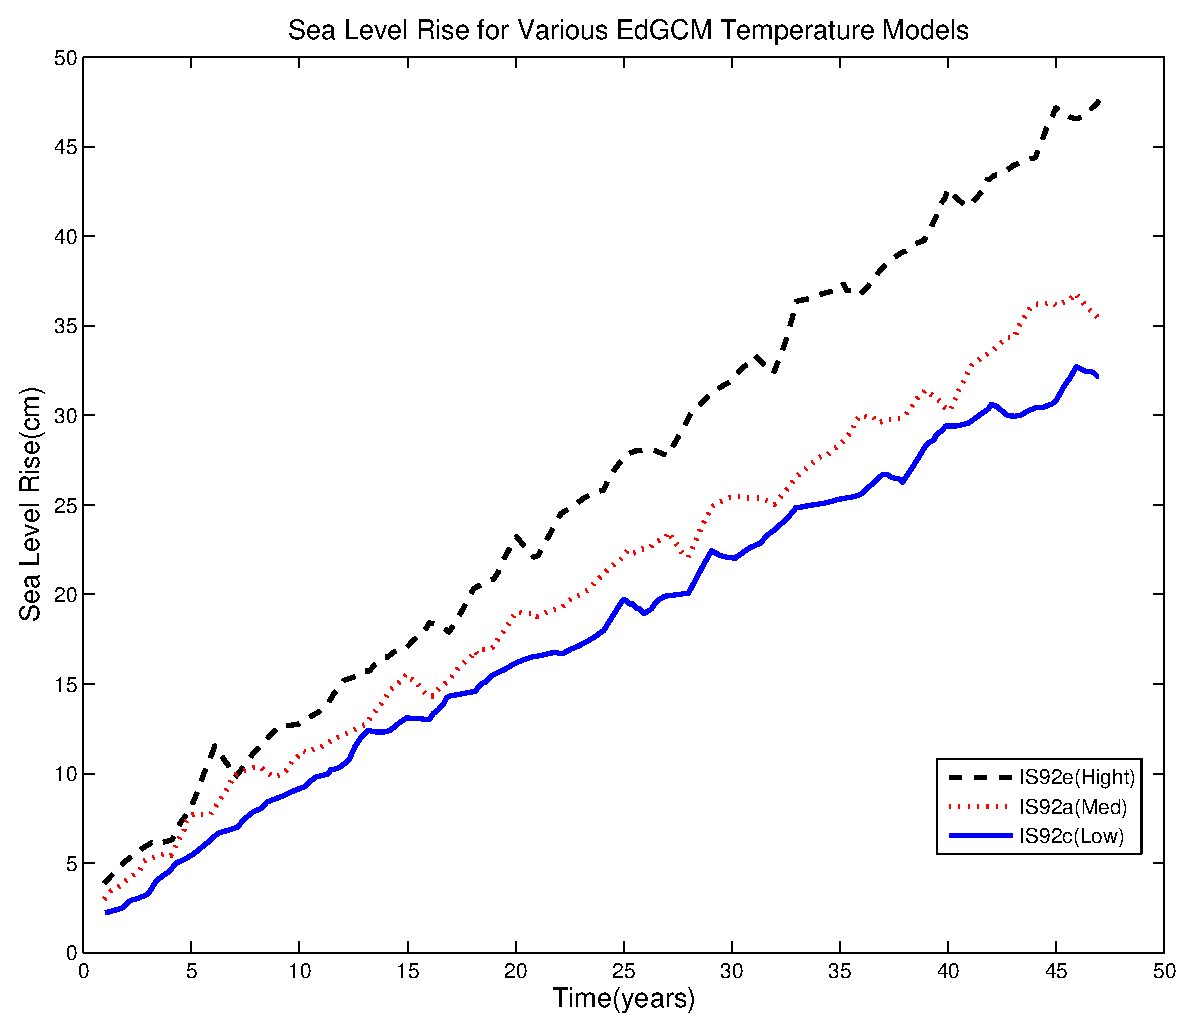
\includegraphics[width=0.8\textwidth]{fig06.eps}
\caption{Sea level rise as a function of time for the three
temperature models}
\end{figure}

Note that the higher temperature corresponds with higher sea level
rise, as we expect it to. The data at the end of 10-year intervals
was recorded and tabulated in Table 1. Units of sea level rise are
in centimeters.

\begin{table}[!htb]
\centering \caption{Sea Level Rise (cm) per Decade for each
Temperature Model}
\begin{tabular}{|l|l|l|l|l|l|}
\hline
 & 10years & 20years & 30years & 40years & 50years \\
\hline
IS92e(Hight) & 12.67  & 23.26  & 31.93  & 41.68  & 46.92 \\
\hline
IS92a(Med) & 11.14        & 18.79    & 25.08  &     30.44  &    36.61  \\
\hline
IS92c(Low) & 9.16  & 16.26  & 21.66  & 29.32  & 32.08 \\
\hline
\end{tabular}
\end{table}

The sea level output data was then used to calculate submersion
consequences. These data were fed as input to the submersion
simulation, detailed in the following section.

\subsection{Submersion Simulation Results}

Submersion information was calculated for each of the three
temperature models during every decade. Output consisted of the
submerged land area and displaced population statistics.

For the IS92e (high) scenario, sea level increases resulted in the
following simulated geographic consequences (shown every decade
for 5 decades):

\begin{figure}[!htb]
\centering
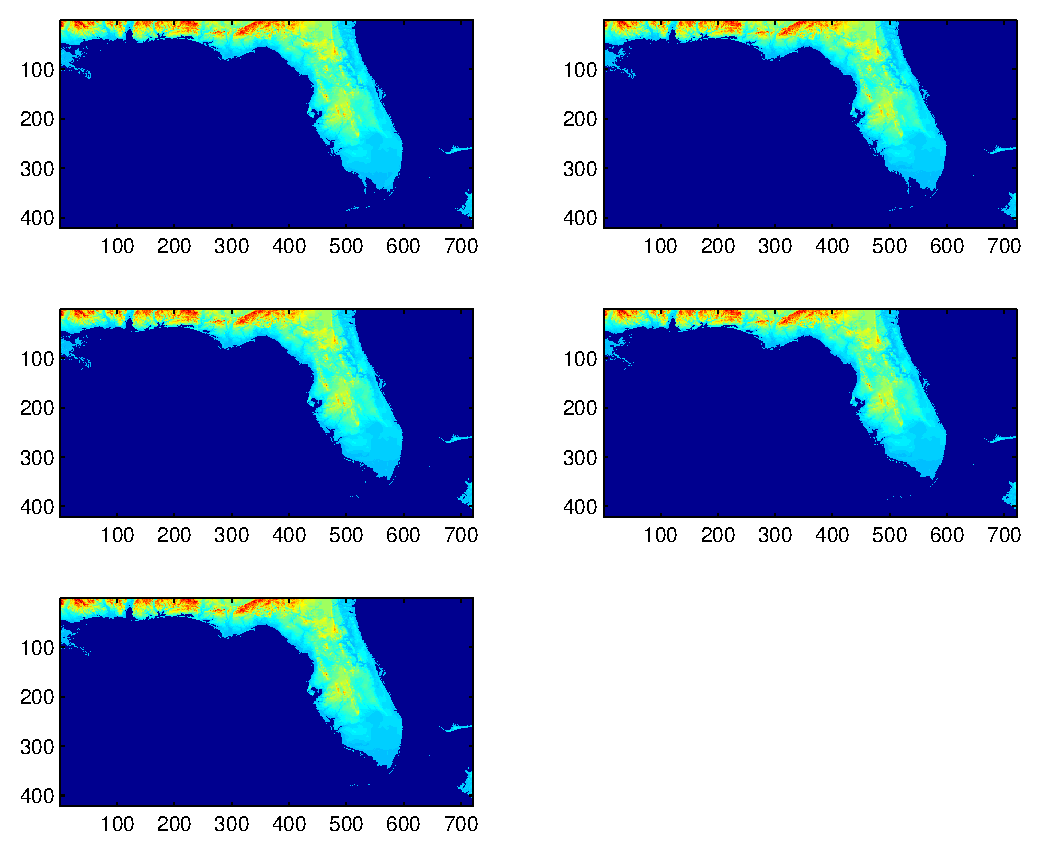
\includegraphics[width=1\textwidth]{fig07.eps}
\caption{Submersion simulation for IS92e}
\end{figure}

Although not much has appeared to have happened, minor topological
changes can clearly be seen at the southern tip of Florida and
parts of Louisiana during the 50 year span. Additionally, the
MATLAB program quantified the following effects:

\begin{table}[!htb]
\centering \caption{Quantitative Effects for IS92E}
\begin{tabular}{|l|l|}
\hline
 & Effects \\
\hline
10years & 0.00e+00 people displaced \\
\hline
 & 6.52e+03 sq km land submerged \\
\cline{2-2}
20 years & Key Largo, FL is submerged: 11886 people \\
 & have been displaced \\
\cline{2-2}
 & have been displaced \\
\hline
30years & Miami Beach, FL is submerged: 87925 \\
 & people have been displaced \\
 & Key Largo, FL is submerged: 11886 people \\
 & have been displaced \\
\hline
 & 9.98e+04 people displaced \\
 & 9.18e+03 sq km land submerged \\
\hline
40years & Merritt Island, FL is submerged: 36090 \\
 & people have been displaced \\
 & Miami Beach, FL is submerged: 87925 \\
 & people have been displaced \\
 & Key Largo, FL is submerged: 11886 people \\
 & have been displaced \\
\cline{2-2}
 & 1.35e+05 people displaced \\
 & 9.97e+03 sq km submerged \\
\hline
50years & Merritt Island, FL is submerged: 36090 \\
 & people have been displaced \\
 & Miami Beach, FL is submerged: 87925 \\
 & people have been displaced \\
 & Key Largo, FL is submerged: 11886 people \\
 & have been displaced \\
\cline{2-2}
 & 1.35e+05 people displaced \\
 & 9.97e+03 sq km submerged \\
\hline
\end{tabular}
\end{table}

\newpage

For the IS92a (Med) scenario, sea level increases resulted in the
following simulated geographic consequences (shown every decade
for 5 decades):

\begin{figure}[!htb]
\centering
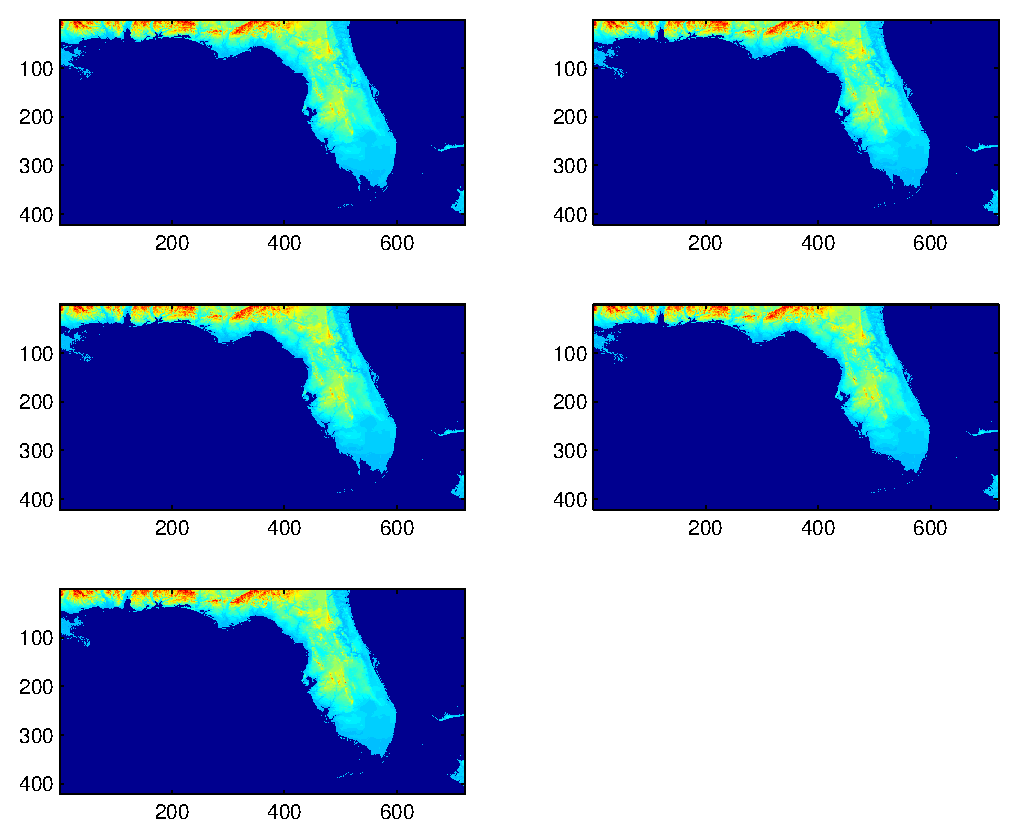
\includegraphics[width=1\textwidth]{fig08.eps}
\caption{Submersion simulation for IS92a}
\end{figure}

\newpage

The overall qualitative damages are comparable to those for IS92e.
MATLAB returned the following damages:

\begin{table}[!htb]
\centering \caption{Quantitative Effects for IS92A}
\begin{tabular}{|l|l|}
\hline
 & Effects \\
\hline
10year & 0.00e+00 people displaced \\
\cline{2-2}
 & 6.43e+03 sq km land submerged \\
\hline
20year & 0.00e+00 people displaced \\
\cline{2-2}
 & 6.94e+03 sq km sq km land submerged \\
\hline
30year & Key Largo, FL is submerged: 11886 people \\
 & have been displaced \\
\hline
 & 1.18e+04 people displaced \\
 & 7.71e+03 sq km land submerged \\
\hline
40year & Miami Beach, FL is submerged: 87925 \\
 & people have been displaced \\
 & Key Largo, FL is submerged: 11886 people \\
 & have been displaced \\
\hline
 & 9.98e+04 people displaced \\
 & 8.96e+03 sq km submerged \\
\cline{2-2}
50year & Miami Beach, FL is submerged: 87925 \\
 & people have been displaced \\
\cline{2-2}
 & Key Largo, FL is submerged: 11886 people \\
 & have been displaced \\
\hline
 & 9.98e+04 people displaced \\
 & 9.46e+03 sq km submerged \\
\hline
\end{tabular}
\end{table}

\newpage

 The key differences for the IS92A data compared to the IS92E
data are that

\begin{enumerate}

\item Key Largo is submerged 10 years later

\item Miami Beach is submerged 20 years later

\item Merritt Island is not submerged after 50 years

\end{enumerate}

Finally, for the IS92c (low) scenario, sea level increases
resulted in the following simulated geographic consequences (shown
every decade for 5 decades):
\begin{figure}[!htb]
\centering
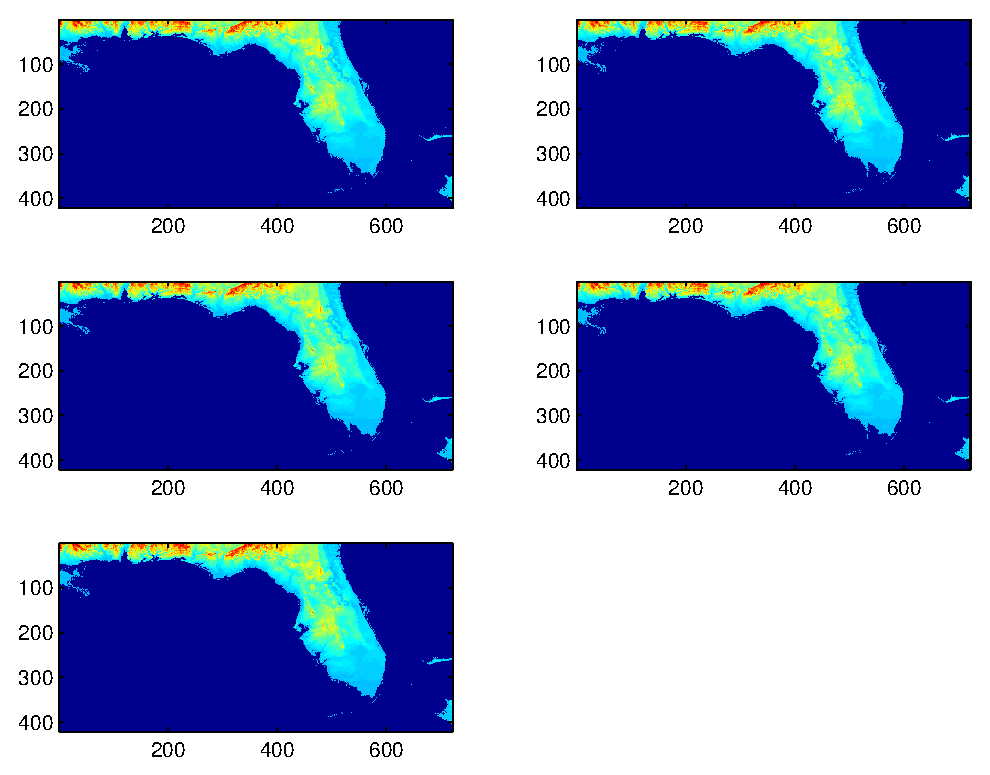
\includegraphics[width=1\textwidth]{fig09.eps} \caption{Submersion simulation for IS92c}
\end{figure}

\newpage

The overall qualitative damages are comparable to those for IS92e
and IS92a. MATLAB returned the following damages:
\begin{table}[!htb]
\centering \caption{Quantitative Effects for IS92A}
\begin{tabular}{|l|l|}
\hline
 & Effects \\
\hline
10years & 0.00e+00 people displaced \\
\cline{2-2}
 & 6.15e+03 sq km land submerged \\
\hline
20years & 0.00e+00 people displaced \\
\cline{2-2}
 & 6.79e+03 sq km land submerged \\
\hline
30years & 0.00e+00 people displaced \\
\cline{2-2}
 & 7.12e+03 sq km land submerged \\
\hline
40years & Miami Beach, FL is submerged: 87925 \\
 & people have been displaced \\
 & Key Largo, FL is submerged: 11886 people \\
 & have been displaced \\
\cline{2-2}
 & 9.98e+04 people displaced \\
 & 7.96e+03 sq km submerged \\
\hline
50years & Miami Beach, FL is submerged: 87925 \\
 & people have been displaced \\
 & Key Largo, FL is submerged: 11886 people \\
 & have been displaced \\
\cline{2-2}
 & 9.98e+04 people displaced \\
 & 9.19e+03 sq km submerged \\
\hline
\end{tabular}
\end{table}


The key differences for the IS92C data compared to the IS92A and
IS92E data is that no metropolitan areas are submerged after 30
years. However, note that in both the IS92A and IS92C scenarios,
Miami Beach and Key Largo are submerged after 40 years.

\section{Discussion and Conclusion}

The estimated sea level rise (shown in Figure 6) for the three
emissions scenarios seems very reasonable. The 50-year projection
is in general agreement with models proposed by the IPCC , NRC,
and EPA (less than 10 cm different from all of them) .
Additionally, the somewhat-periodic, somewhat-linear trend is
similar to past data of mean sea level rise collected in various
locations . Thus, the projections made by our model are feasible.

The high emission scenario results in about $40\sim 50cm$ rise in
sea level by 2058, with results from the intermediate scenario
$6\sim 10cm$ below that and the low emission scenario

trailing intermediate by $5\sim 8cm$. The model thus works as we
expected for a wide range of input data; higher temperatures
should lead to increased sea level rise.

Overall, the damage due to sea level change seemed unremarkable.
Even in our "worst case scenario," in 50 years only approximately
200,000 people are displaced, and 10,000 square kilometers are
submerged-mostly from the South Florida metropolitan area and
other coastal regions. The effects could barely be visualized on
the submersion simulation.

However, these projections are only the beginning of what could be
a long-term trend. As shown by the control results, a sea level
increase of 10 meters would be devastating. Further, not all
possible damages could be assessed in our simulation. For example,
sea level increases have been directly implicated in shoreline
retreat, erosion, and saltwater intrusion, which were not
quantified in our model. Economic damages also could not be
directly assessed. Global warming presents a very complex
economics problem. Bulkheads, levees, seawalls, and other manmade
structures are often utilized to counteract the effect of rising
sea levels, and their economic impacts are outside the scope of
the model. High-resolution economic data is also required, to
determine the value of the threatened land.

Our model has several key limitations. The core assumption of the
model is the simplification of physical features and dynamics in
Greenland. The model assumes an environment where thickness,
temperature, and other physical properties of interest are
averaged out and evenly distributed. And then the "sublimate, melt
and snow" dynamics are simulated on a monthly time step is
employed. Such assumptions are obviously far too simplistic to
fully capture the ongoing dynamics in the ice sheets. But without
the tremendous data and computing power required to perform a
full-scale 3-D grid-based simulation using energy-mass balance
models, such as in , an alternative had to be pursued.

With regards to more minor details of the model, the assumed
properties regarding the thermal expansion, localization, and
accumulation also take an averaging approach towards evaluating
the geological trends. As mentioned in previous sections,
understanding, let alone simulating, these phenomena and methods
with a high degree of accuracy is difficult due to their innate
complexities. An empirical estimate is often made in literatures,
such as one we adapted from , and thus we occasionally adopt
simplified models. However, because of these empirical approaches,
our model may not hold over extremely long periods of time, where
models for accumulation, thermal expansion, and localization might
break down.

A discussion of the emission scenarios, the heart of the input
data, is also relevant. The data is a subset of simulation result
using IS92 emission scenarios on EdGCM model, the core of which is
the GISS-II GCM (Global Climate Model) developed by NASA . The
assumptions of the EdGCM model are fairly minimal for computing on
a desktop, and the projected temperature time series associated
with each scenario-high, medium, and low-were consistent with
typical carbon projections . Although the IS92 emissions scenarios
are very rigorous, they are the main weakness of the model.
Because all of the other parameters are dependent on the
temperature model, our results are particularly sensitive to
factors that directly affect the EdGCM output. This situation is
complicated further by the fact that an explicit-form solution
cannot be obtained with our mathematical foundation. The variable
we solve for is inside the Fourier series term and requires
sophisticated numerical computations to approximate; thus, we
cannot directly assess the dependence of sea level rise on
temperature.

Despite these deficiencies, our model is an extremely powerful
tool for climate modeling. The relative simplicity, while it can
be viewed as a weakness, is actually a key strength of the model.
The model boasts rapid run-time in comparison with its more
sophisticated peers due to the simplifications of variables.
Furthermore, the model is basically a function of time and
temperature only. The fundamentals of our model imply that all of
the sea level increases are due to temperature change; this
relationship is obscured in other models involving a large amount
of independent variables. But even with less complexity, the model
is comprehensive and accurate enough to produce quality results
and provide accurate predictions. Indeed, as we have shown, the
predictions of our model closely parallel past data. Additionally,
the associated visualization tool allows for easy recognition of
the sea level rise effects in Florida.

\section{Recommendations}

In the short term, preventative action could spare many of the
submersion model's predictions from becoming a reality. Key Largo
and Miami Beach in particular were identified as particularly
vulnerable. These regions act as a buffer zone, preventing
salinization of interior land and freshwater. If these regions
flood, seawater intrusion may occur, resulting in widespread
ecological, agricultural, and ultimately economical damage.

One possible action is to build sand walls around the South Beach
shoreline. In order to provide a basic cost-benefit analysis, we
plan to construct a 0.5 $m$ sand structure (estimated by our model
to provide at least 50 years of safety) protecting the shoreline
of Miami Beach (about 5 $km$). A standard with of such a structure
is 20$m$. Assuming that we obtain all of the sand from 0$\sim$1
mile offshore, then the cost is given by

\[
\$4/yd^3\cdot\frac{5000m\cdot20m\cdot1yd^2}{(0.9114m)^2}\cdot\frac{0.5m}{1yd/0.9114m}=\$264,182
\]

according to projections from Titus et al . Clearly, the financial
damage from coastal flooding in the absence of the coastal
protection will far outweigh the cost of constructing the
necessary coastal protection facilities (dunes/seawalls). Using
the same reasoning, protective structures must be constructed
around Key Largo.

If greenhouse gas emissions continue to increase dramatically,
construction of the sand wall will be impractical. A long term
solution, reducing carbon emissions globally, is required to
ultimately protect low-elevation coastal regions. As our model
shows, decreased carbon emissions result in significant slowing of
sea level rise, even on a 50- year timescale. In the long run,
carbon emissions must be reduced in order to prevent disasters
associated with sea level rise.

\newpage
\begin{thebibliography}{1}

\bibitem{1}

\bibitem{2}

\bibitem{3}

\end{thebibliography}
\newpage



\section{Appendix}

\subsection{Appendix A Sea Level Rise Simulation Script}

\lstinputlisting[language=matlab]{./A.m}

\newpage
\subsection{Appendix B Topological Raster Matrix Creation Script}

\lstinputlisting[language=matlab]{./B.m}

\newpage
\subsection{Appendix C Submersion Simulation Script}
\lstinputlisting[language=matlab]{./C.m}

\newpage

\subsection{Appendix D Florida Cities Data Initialization}
\lstinputlisting[language=matlab]{./D.m}

\end{document}
